\section{Entwurf}

\subsection{Use-Cases}

\subsection{Technologien}


\subsection{Systemarchitketur}
Bei der Systemarchitektur fiel die Wahl auf eine Server-Client Anwendung. Aufgrund der Anforderung ein Monitoring-System zu erstellen, sprich der Nutzer über eine grafische Schnittstelle bestimmte Werte angezeigt bekommen lassen möchte, musste ein Client erstellt werden. Weiterhin war gefordert, dass Sensoren von verschiedenen Haushalten aus Daten an das Monitoring-System schicken und diese auch gespeichert werden. Daher musste es eine Möglichkeit geben, die Daten von verschiedenen Quellen in einer zentralen Einheit verwalten zu können. Hierfür wurde ein Server mit angebundener Datenbank ausgewählt. Hieraus entstand der folgende erste Entwurf der Systemarchitektur:

\begin{figure}[h]
\begin{center}
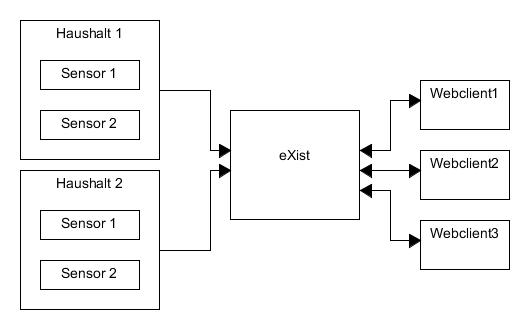
\includegraphics[scale=0.7]{images/sa1.jpg} 
\caption{Erster Entwurf Systemarchitektur}
\end{center}
\end{figure}

Ein eXist-Server stellt dabei die zentrale Komponente dar, die sowohl alle Daten von den Sensoren entgegennimmt und verwaltet, sowie auch für die Kommunikation zwischen dem Server und den Clients verantwortlich ist. Für die Sensoren stellt der Server einen REST-Service zur Verfügung, welcher als Übertragungsschnittstelle der ermittelten Vitalwerte dient. So ist es auch leicht möglich, weitere Sensoren an das System anzuschließen, da lediglich die Adresse des REST-Services bekannt sein muss und in welcher Form die Daten übertragen werden müssen. Ansonsten gibt es keine direkte Kopplung. Für die Kommunikation zwischen Server und Clients hätte ebenfalls ein REST-Service verwendet werden können. Hierbei hätte sich jedoch das Problem ergeben, dass sich die Daten von den Sensoren in sehr kurzen Zeitabständen ändern. Um jedoch immer die aktuellsten Vitalwerte anzeigen zu können, müsste der Client sehr oft den Server nach neuen Daten abfragen. Bei mehreren Clients könnte dies zu einer Serverüberlastung führen, da der Server nicht mehr alle Anfragen in kurzer Zeit beantworten kann.
\\
\\
Daher wurde entschieden, die Kommunikation mittels Websockets zu realisieren. Der Vorteil besteht darin, dass der Client nur einmal die Verbindung zum Server aufbaut und dieser dann die Verbindung nutzt, um Daten an den Client zu schicken ohne das dieser sich neu verbinden muss. Dies eignet sich besonders gut für das Monitoring-System: Sobald die Sensoren neue Daten schicken, können diese direkt an den wartenden Client weitergeleitet werden, der bereits die Verbindung geöffnet hat und in dem Sinne empfangsbereit für jede Änderung ist. Mit eXist ist eine solche Kommunikationsart nicht möglich, da es keine solche Implementierung der Websockets besitzt. Aus diesem Grund wurde ein zweiter Server hinzugenommen, der sowohl eine REST-Schnittstelle als auch Websockets zur Verfügung stellt. Die Wahl fiel dabei auf einen Node.JS-Server, da dieser sehr ressourcensparend ist und viele gleichzeitige Netzwerkverbindungen ermöglicht. Der neue Entwurf für die Systemarchitektur ist nun wie folgt:

\begin{figure}[h]
\begin{center}
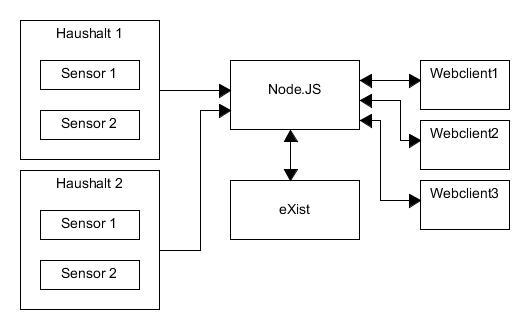
\includegraphics[scale=0.7]{images/sa2.jpg} 
\caption{Zweiter Entwurf Systemarchitektur}
\end{center}
\end{figure}

Der Node.JS-Server ist nun die zentrale Einheit und steuert die Kommunikation zwischen den Sensoren und den Clients. Weiterhin speichert er alle empfangenen Werte in der eXist-Datenbank ab. Hauptsächlich besteht die Aufgabe des Node.JS-Servers darin, die Anfragen und Antworten an die entsprechenden Stellen (eXist, Client) weiterzuleiten. Dies war jedoch nötig, um sowohl REST-Services, als auch Websockets verwenden zu können.

\subsection{Kommunikation}
Die Sensoren schicken ihre ermittelten Werte (\textit{sensorData}) an den Node.JS -Server. Dabei wird die Antwort vom Server jedoch ignoriert, da von den Sensoren keine  Fehlerbearbeitung vorgesehen ist. Die Daten werden über eine REST-Anfrage (POST) mit dem entsprechenden XML-Dokument gesendet.

\begin{figure}[h]
\begin{center}
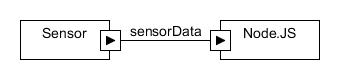
\includegraphics[scale=0.8]{images/komm1.jpg} 
\caption{Kommunikation zwischen Sensoren und Node.JS-Server}
\end{center}
\end{figure}

Der eXist-Server bietet zur Kommunikation einen Standard, mit dem sich mittels XQuery REST-Services erstellen lassen. \textit{RESTXQ} bietet verschiedene Annotation, um beispielsweise einen URL-Pfad anzugeben, unter der eine Funktion von außerhalb angesprochen werden kann, oder um die Funktion als eine POST-Methode festzulegen. Mit Hilfe der Annotationen wurde nun die Kommunikation zwischen dem Node.JS-Server und der eXist-Datenbank hergestellt. Die von den Sensoren empfangenen Daten werden mittels POST an die Datenbank geschickt (\textit{sensorData}). Weiterhin kann mittels einem \textit{reportRequest} ein Report für eine bestimmte Person in einem Zeitraum über alle Vitalwerte angefordert werden. Der eXist sendet daraufhin die erstellte PDF-Datei als \textit{reportData} wieder zum Node.JS-Server. Außerdem kann geprüft werden, ob eine \textit{personId} in der Datenbank bereits verzeichnet ist. Dafür sendet der Node.JS-Server eine Anfrage mit der \textit{personId} an eXist und erhält eine Meldung über die Existenz der ID (\textit{personIdResponse}).

\begin{figure}[h]
\begin{center}
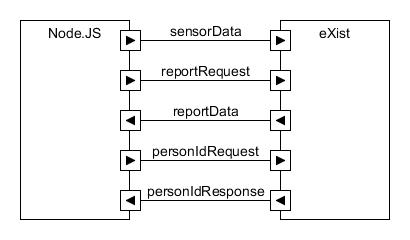
\includegraphics[scale=0.8]{images/komm2.jpg} 
\caption{Kommunikation zwischen Node.JS-Server und eXist}
\end{center}
\end{figure}

Von den Clients aus können sowohl die Reports, als auch die Überprüfung der gewünschten \textit{personId} angefordert werden. Der Node.JS-Server leitet diese Anfragen an eXist weiter und gibt die Antworten an die Clients zurück. Diese Anfragen hätten auch über einen REST-Service erstellt werden können, man entschied sich aber dafür, die Kommunikationsarten auf Clientseite nicht zu vermischen. Außerdem erhält der Client über die offene Websocket-Verbindung jeden neuen Wert, der von den Sensoren geschickt wurde.  

\begin{figure}[h]
\begin{center}
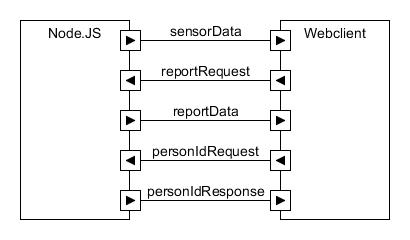
\includegraphics[scale=0.8]{images/komm3.jpg} 
\caption{Kommunikation zwischen Node.JS-Server und Client}
\end{center}
\end{figure}